\scanpage{346}
\mspage{175}

We observe that, with the exception of the two homogeneous spaces
(under $\widehat{\widehat{\mathcal G}}(\pi)$, but not \unsure{necessarily|necessarily} under
$\widehat{\widehat{\mathcal G}}(\pi,I')$, or even under
$\widehat{\widehat{\mathcal G}}^{!}(\pi)$) Bases $(\pi)$ and Outer bases $(\pi)$,
the other four are in fact homogeneous spaces under
$\widehat{\widehat{\mathcal G}}^{!}$, and are expressed as quotients of the
\inserted{$\widehat{\widehat{\mathcal G}}^{!}_{g,\nu}$-}torsor
$\operatorname{Isom}^{!}(\widehat{\pi}_{g,\nu},\pi)$, by the four subgroups
\[
\mathcal G^{!}_{g,\nu},\quad
\mathcal G^{!}_{g,\nu}\cdot\widehat{\pi}_{g,\nu},\quad
\widehat{\mathcal G}^{!}_{g,\nu},\quad
\mathcal M^{!}_{g,\nu}
\]
(the last defined as the inverse image of $\mathcal N^{!}_{g,\nu}$ in
$\widehat{\widehat{\mathcal G}}_{g,\nu}$, just as $\mathcal M_{g,\nu}$ is defined
as the inverse image of $\mathcal N_{g,\nu}$).
We find on the other hand, \unsure{if|for} $I'=\{i_0,\ldots,i_{\nu'-1}\}$,
\unsure{a|some} homomorphism
\[
\widehat{\widehat{\mathcal G}}^{!}_{g,\nu}\longrightarrow
\widehat{\widehat{\mathcal G}}^{!}_{g,\nu'},
\]
sending $\mathcal G^{!}_{g,\nu}$ into $\mathcal G^{!}_{g,\nu'}$,
\deleted{\illegible{1} $\unsure{\widehat{\mathcal G}}_{g,\nu}$ into
$\unsure{\widehat{\pi}_{g,\nu}}$}
by sending $\pi_{g,\nu}$ into $\pi_{g,\nu'}$, thus $\widehat{\pi}_{g,\nu}$
into $\widehat{\pi}_{g,\nu'}$,
$\widehat{\mathcal G}^{!}_{g,\nu}=\Sigma^{!}_{g,\nu}$ into
$\widehat{\mathcal G}^{!}_{g,\nu'}=\Sigma^{!}_{g,\nu'}$, and the subgroup
$\mathcal G^{!}_{g,\nu}\cdot\widehat{\pi}_{g,\nu}$ of
\deleted{\illegible{1}} \inserted{$\widehat{\mathcal G}^{!}_{g,\nu}$}
into the subgroup $\mathcal G^{!}_{g,\nu'}\cdot\widehat{\pi}_{g,\nu'}$ of
$\widehat{\mathcal G}^{!}_{g,\nu'}$.
Finally, since $\Sigma^{!}_{g,\nu}$ maps into $\Sigma^{!}_{g,\nu'}$,
\deleted{\illegible{1}} $\mathcal N^{!}_{g,\nu}$ maps into the normalizer
of $\Sigma^{!}_{g,\nu'}$ \inserted{(in $\widehat{\widehat{\mathcal T}}^{!}_{g,\nu'}$)},
\deleted{which}\inserted{I say that this} is none other than $\mathcal N^{!}_{g,\nu'}$.
Changing notation, this amounts to the

\uline{Lemma}\quad The
$\mathcal N^{!}_{\Sigma}=\operatorname{Norm}_{\widehat{\widehat{\mathcal T}}^{!}}(\Sigma^{!})$
\deleted{\illegible{1}}
$\bigl(=\operatorname{Norm}_{\widehat{\widehat{\mathcal T}}}(\Sigma^{!})\cap
\widehat{\widehat{\mathcal T}}^{!}\bigr)$.

\margin{not proved\quad
\deleted{\illegible{4} of
$\unsure{\operatorname{Norm}_{\widehat{\widehat{\mathcal T}}}(\Sigma^{!})/\Sigma^{!}}$}}

Obviously we have
$\mathcal N^{!}_{\Sigma}\subset
\operatorname{Norm}_{\widehat{\widehat{\mathcal T}}}(\Sigma^{!})\cap
\widehat{\widehat{\mathcal T}}^{!}$,
conversely let $g\in\widehat{\widehat{\mathcal T}}^{!}$ which normalizes
$\unsure{\Sigma^{!}}$, let us show that it normalizes $\Sigma$ i.e.
that it \unsure{is} $\in\mathcal N$
(thus $\in\mathcal N^{!}=\mathcal N\cap\widehat{\widehat{\mathcal T}}^{!}$).
\mspage{345}

\scanpage{347}

It's not clear. I \inserted{nevertheless} feel like \unsure{proving|pronouncing} \deleted{\illegible{1}} the
\uline{conjecture} The canonical map
\[
\unsure{\text{Prediscretifications}|\text{Prediscretifications}}^{+}(\pi)
 \overset{\sim}{\longrightarrow}
\unsure{\text{Prediscretifications}|\text{Prediscretifications}}^{+}(\pi')
\]
is \uline{bijective}. In order \inserted{that} two \unsure{oriented} prediscretifications
$\alpha,\beta$ of $\pi$ \deleted{\unsure{be}} \unsure{have} the same group of outer \unsure{automorphisms}
$\Sigma_\alpha=\Sigma_\beta$, \deleted{then} it is necessary and \unsure{sufficient}
\deleted{\unsure{for their images}} \inserted{that it be so.}
for their images $\Sigma_{\alpha'}$ and $\Sigma_{\beta'}$, i.e. that
$\Sigma_{\alpha'}=\Sigma_{\beta'}$; so that the preceding bijection induces a bijection
\[
\text{Prearithmetizations}(\pi)\overset{\sim}{\longrightarrow}\text{Prearithmetizations}(\pi').
\]
Finally, \deleted{the map $\widehat{\widehat{\mathcal T}}(\pi)\longrightarrow
\widehat{\widehat{\mathcal T}}(\pi')$, which induces}
\inserted{the preceding bijections are compatible with}
the homomorphism of the groups \inserted{of operators}
$\widehat{\widehat{\mathcal T}}(\pi,I')\longrightarrow\widehat{\widehat{\mathcal T}}(\pi')$,
\deleted{\unsure{which induces}} \inserted{a fortiori}
a $\widehat{\widehat{\mathcal T}}^{!}(\pi)\longrightarrow\widehat{\widehat{\mathcal T}}^{!}(\pi')$,
\deleted{this} which implies \unsure{that it thereby induces|that it induces them}
(for a given prearithmetization $\Sigma$ \inserted{$\subset\widehat{\widehat{\mathcal T}}(\pi)$}
of $\pi$, giving $\Sigma'$ \inserted{$\subset\widehat{\widehat{\mathcal T}}(\pi')$}
in $\pi'$; \inserted{with $\Sigma^{!}\longrightarrow\Sigma'^{!}$}) a
homomorphism
$\mathcal N_\Sigma^{!}\deleted{\unsure{(\Sigma)}}\longrightarrow
\mathcal N_{\Sigma'}^{!}\deleted{\unsure{(\Sigma')}}$,
\deleted{\unsure{which is likewise}} and the \unsure{corresponding} homomorphism
\[
\Gamma_\Sigma=\deleted{\widehat{\widehat{\mathcal T}}}\mathcal N_\Sigma^{!}/\Sigma^{!}
 \longrightarrow
\deleted{\unsure{\mathcal N_{\Sigma'}^{!}/\Sigma'^{!}}}\Gamma_{\Sigma'}=\mathcal N_{\Sigma'}^{!}/\Sigma'^{!}
\]
is an isomorphism.

To convince oneself of this it suffices to look at
\deleted{\unsure{$\pi=\widehat{\pi}_{g,\nu}$}}
\inserted{(\unsure{choosing} $\pi=\unsure{\pi_{g,\nu}|\widehat{\pi}_{g,\nu}}$,
$I'$ \deleted{\illegible{1}} \unsure{reduced to the|being a} last \unsure{element|element} of $I_\nu$)}
the case where $I'=\{\unsure{i'|i}\}$, We then have a homomorphism
\[
\widehat{\widehat{\mathcal T}}(\pi,i)\longrightarrow
\widehat{\widehat{\mathcal G}}(\pi').
\]
(the \uline{outer} automorphisms with loops of $\pi$ fixing $i$ define
well-determined \unsure{automorphisms} of $\pi'$ --- not just outer ones)
\mspage{346}

\scanpage{348}
\mspage{176}

i.e. $\widehat{\widehat{\mathcal G}}(\pi,i)\longrightarrow
\widehat{\widehat{\mathcal G}}(\pi')$ is trivial on $\unsure{\widehat{\pi}}$, and
thus passes to the quotient as a
$\widehat{\widehat{\mathcal T}}(\pi,i)\longrightarrow
\widehat{\widehat{\mathcal G}}(\pi,i)$.
I assume, \deleted{that} by analogy with the discrete case,
that this homomorphism is an \uline{isomorphism}, so that we have an exact sequence
\margin{\figure{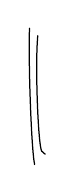
\begin{tikzpicture}[x=1cm,y=1cm,line width=.45pt,line cap=round]
\draw (0,0) .. controls (-.015,-.48) and (.025,-1.54) .. (.065,-1.73);
\draw (.105,-.095) .. controls (.070,-.48) and (.110,-1.48) .. (.155,-1.56) .. controls (.165,-1.58) and (.185,-1.59) .. (.200,-1.60);
\end{tikzpicture}}}
\margin{\unsure{recall that we assume} $\pi$ \unsure{anabelian|nonabelian}
$(2g+\nu\geq3)$}
\[
1\longrightarrow\pi'\longrightarrow
\widehat{\widehat{\mathcal T}}(\pi,i)\longrightarrow
\unsure{\widehat{\widehat{\mathcal G}}}(\pi',i)\longrightarrow1
\]
or again
\[
1\longrightarrow\widehat{\pi}_{g,\nu-1}\longrightarrow
\widehat{\widehat{\mathcal T}}_{g,(\nu,\nu-1)}
\longrightarrow\unsure{\widehat{\widehat{\mathcal G}}}_{g,\nu-1}
\longrightarrow1
\]
which contains the exact sequence
\[
1\longrightarrow\pi_{g,\nu-1}^{\unsure{*|+}}\longrightarrow
\mathcal T_{g,(\nu,\nu-1)}\longrightarrow
\unsure{\mathcal G}_{g,\nu-1}\longrightarrow1
\]
\unsure{as|known} sub\deleted{\unsure{particular|dense part}}, \unsure{sequence|is} exact.
It is convenient to work instead with
\diagram{\begin{tikzcd}[ampersand replacement=\&,column sep=2.1em,row sep=3.0em]
1 \arrow[r,dash] \&
\pi_{g,\nu-1} \arrow[r,dash] \arrow[d,hook',no head] \&
\unsure{\mathcal T}_{g,\nu}^{!+} \arrow[r] \arrow[d,hook',no head] \&
\mathcal G_{g,\nu-1}^{!+} \arrow[r,dash] \arrow[d,hook',no head] \& 1 \\
1 \arrow[r,dash] \&
\widehat{\pi}_{g,\nu-1} \arrow[r] \arrow[d,equal] \&
\underset{\deleted{\unsure{\illegible{1}}}}{\widehat{\mathcal T}_{g,\nu}^{!+}}
\arrow[r] \arrow[d,hook',no head] \&
\widehat{\mathcal G}_{g,\nu-1}^{!+} \arrow[r,dash] \arrow[d,hook'] \& 1 \\
1 \arrow[r,dash] \&
\widehat{\pi}_{g,\nu-1} \arrow[r] \&
\widehat{\widehat{\mathcal T}}_{g,\nu}^{!} \arrow[r] \&
\widehat{\widehat{\mathcal G}}_{g,\nu-1}^{!} \arrow[r,dash] \& 1
\end{tikzcd}}

The map $\unsure{\text{Prediscretifications}|\text{Prediscretifications}}^{+}(\pi)\longrightarrow
\unsure{\text{Prediscretifications}|\text{Prediscretifications}}^{+}(\pi')$ is thus identified with
$\widehat{\widehat{\mathcal T}}_{g,\nu}^{!}/\widehat{\mathcal T}_{g,\nu}^{!}$,
we read off the diagram that this is
$\simeq\widehat{\widehat{\mathcal G}}_{g,\nu-1}^{\unsure{!}\deleted{\unsure{+}}}/
\widehat{\mathcal G}_{g,\nu-1}^{!+}$,
whence bijectivity on the sets of oriented prediscretifications.

In the group $\widehat{\widehat{\mathcal T}}_{g,\nu}^{!}=\mathcal T$,
we have an invariant subgroup $\widehat{\pi}_{g,\nu-1}=\pi'$,
and a subgroup $\Sigma$ $(\unsure{=|\longleftarrow}\widehat{\mathcal T}_{g,\nu}^{!+})$
\mspage{347}

\scanpage{349}

between $\pi'$ and $\mathcal T$, \deleted{\unsure{giving by}} \inserted{giving} a subgroup $\Sigma'\simeq\mathcal T(\pi')$\inserted{$(=\unsure{\widehat{\mathcal G}^{!+}_{g,\nu-1}})$} in $\unsure{\mathcal T'}=\mathcal T/\pi'$ $(\simeq\widehat{\widehat{\mathcal G}}^{!}_{g,\nu-1})$, and we know well that then
\[
\mathcal T/\Sigma\simeq\mathcal T'/\Sigma',
\]
and \deleted{$\unsure{N(\Sigma)}$} that the normalizer \inserted{$\mathcal N$,} of $\Sigma$ in $\mathcal T$ is the inverse image of the normalizer $\mathcal N'$ of $\Sigma'$ in $\mathcal T'$, so that $\mathcal N/\Sigma\simeq\mathcal N'/\Sigma'$, which proves what we wanted.

\uline{Corollary} We have canonical \unsure{isomorphisms}
\[
\Gamma_{g,\nu}\xrightarrow{\sim}\Gamma_{g,\nu-1}\xrightarrow{\sim}\unsure{\cdots}\quad\deleted{\unsure{\Gamma_{g,0}}}
\]
\margin{We also see that $\unsure{\Sigma|\Sigma^{!}}$ invariant in $\unsure{\mathcal T|\widehat{\widehat{\mathcal T}}}$ is equivalent to $\Sigma'$ invariant in $\widehat{\widehat{\mathcal T}}'$}
so that if $g\geq2$, we have \unsure{canonically} $\Gamma_{g,\nu}\simeq\Gamma_{g,0}$, on the other hand $\Gamma_{1,\nu}\simeq\Gamma_{1,1}$ $(g=1,\nu\geq1)$, $\Gamma_{0,\nu}\simeq\Gamma_{0,3}$ $(\nu\geq3)$.

\uline{N.B.} The ``fact'' \deleted{\illegible{1}} assumed is far from obvious --- even that $\widehat{\widehat{\mathcal T}}^{\unsure{!}}_{g,(\nu,\nu-1)}\longrightarrow\unsure{\widehat{\widehat{\mathcal T}}_{g,\nu-1}|\widehat{\widehat{\mathcal M}}_{g,\nu-1}}$ is surjective, or that $\widehat{\widehat{\mathcal T}}_{g,(\nu,\nu-1)}\longrightarrow\widehat{\widehat{\mathcal G}}_{g,\nu-1}$ is injective, is far from obvious, and is perhaps altogether false !

The assumed fact amounts to a statement of the existence of a functor \unsure{in} the opposite direction ``drilling holes'', \unsure{which|what} in any case remains not understood.

\mspage{348}

\scanpage{350}
\mspage{177}

28. \uline{Change of type} $(g,\nu)$ \unsure{(continued)} : \uline{\unsure{passage} to a finite covering.}

Let $\pi$ be a profinite group \inserted{with loops} of type $(g,\nu)$, anabelian as always, $\pi'$ a subgroup of finite index. We know (\unsure{or we|we thereby} verify, by passing to the discrete case) that \deleted{\illegible{1} \unsure{discretified}} \inserted{equipped with the} \unsure{traces} \unsure{on|under} $\pi$ of the \unsure{loop} subgroups of $\pi$, $\pi'$ is a group with loops.

\deleted{If for every $i\in I(\pi)$, we consider an $L_i$, and the $\unsure{n}$ conjugates $\unsure{\operatorname{int}(g)}L_i$ \inserted{$=L_{i\alpha}$}, with $g\in\pi\bmod\pi'$ $(n=[\pi:\pi']\unsure{\}},\ \deleted{\unsure{n}}\ \inserted{1\leq\alpha\leq n})$ \deleted{\unsure{counted|to count} the number of times that a conjugacy class in $\pi'$ of the subgroup $\unsure{\operatorname{int}(g)}L_i$ is} \inserted{then if $\unsure{d_{\alpha}|d_{i\alpha}}=[L_{i\alpha}:\unsure{L'_{i\alpha}|N'_{i\alpha}}\deleted{\unsure{\cap\pi'}}]$ \unsure{for} $L'_{i\alpha}=L_{i\alpha}\cap\pi'$, then} exactly $d_{i\alpha}$ among the $L'_{i\beta}$ \inserted{$(1\leq\beta\leq n)$} are conjugate in $\pi'$ to $L'_{i\alpha}$, and if we sum over the distinct \unsure{conjugacy} classes of the subgroups}

The loop subgroups are \unsure{also|thus} the \deleted{\unsure{the}} subgroups $L'$ such that
\[
\text{a)}\quad L'=\operatorname{Centr}_{\pi}(L')\cap\pi'.
\]
\[
\text{b)}\quad L\unsure{=|:}\operatorname{Centr}_{\pi}(L')\text{ is a \unsure{loop} subgroup in }\pi.
\]
We put $d(L')=[L:L']$, and we thus have a function
\[
d:I'=I(\pi')\longrightarrow\mathbb N^*,
\]
and a map $I'\xrightarrow{\varphi}I$, such that $\forall i\in I$, we have
\[
\text{(1)}\qquad \sum_{\substack{i'\in I'\\\text{over }i}}d(i')=n
\qquad (\text{\unsure{where|here}}\ n=[\pi:\pi'])
\]
We will have the Hurwitz formula
\[
\text{(2)}\qquad \deleted{\unsure{2g|2\alpha}}\ 2g'-2=n(2g-2)+\overbrace{\sum_{i'\in I'}(d(i')-1)}^{\inserted{n\operatorname{card}I-\operatorname{card}I'}}
\]
\mspage{349}